\chapter{Interferometry}
\label{ch_interferometry}

% In this chapter, I introduce the basic principles of radio interferometry that are relevant to this project. The basic principles include \add{}. I also describe the calibration and imaging steps that are used to process the data. These steps provide the outline for the ALMA data methods described in in Chapter \ref{ch_data}. 


% ------------------------------------------------
\section{Introduction to Interferometers}
% ------------------------------------------------
Studying protostellar disks at millimetre wavelengths requires high-angular-resolution observations to probe their structure through the surrounding protostellar envelope. Because protostellar disks are typically located hundreds of parsecs away, they appear very small in the sky, and the angular resolution is limited by diffraction. The angular resolution, $\theta_{\text{res}}$, of a single-dish radio telescope observing at wavelength $\lambda$ is approximately:
\begin{equation}
    \theta_{\text{res}}\sim \lambda/D,
\end{equation}
\noindent where $D$ is the diameter of the dish \citep{Monnier}. Achieving the angular resolution required to study a protostellar disk with a single-dish telescope would therefore require an impractically large dish. For example, IRS~63 is located $\sim$ 144 parsecs away, and to resolve its structure on scales $< 50$ au requires an angular resolution of $<$ 0.5 arcsec. At millimetre wavelengths, achieving this resolution would require a telescope around a kilometre in diameter. 


To overcome this limitation, radio astronomers use interferometers, which combine observations from multiple widely separated dishes to synthesize a large dish, improving angular resolution  \citep{Ludovici2026}. The angular resolution of an interferometer is:
\begin{equation}
    \theta_{\text{res}}\sim \lambda/B, 
\end{equation}
\noindent where $B$ is the maximum distance between two telescopes, known as the baseline \citep{Monnier}. 
% ------------------------------------------------








% ------------------------------------------------
\section{The Basics of Interferometry}
% ------------------------------------------------
% The simplest interferometer consists of two telescopes that observe the same astronomical object.

When the signals from a pair of antenna arrive at the correlator to be combined, they either have constructive or destructive interference, producing a larger or smaller wave, respectively \citep{Monnier}. Because the antennas are separated by some distance, radio waves from the astronomical source reach the antennas at different times, producing a geometric delay between the signals, as shown in Figure \ref{fig: path-delay}. The signals collected by the two antennas are combined to create an interference pattern, known as a fringe. Longer baselines make finer fringes and provide higher angular resolution information, making the interferometer sensitive to smaller-scale structures. Alternatively, shorter baselines make larger fringes, which are lower in angular resolution but are more sensitive to larger-scale structure \citep {Perley2026}. 
\begin{figure}[htbp]
    \centering
    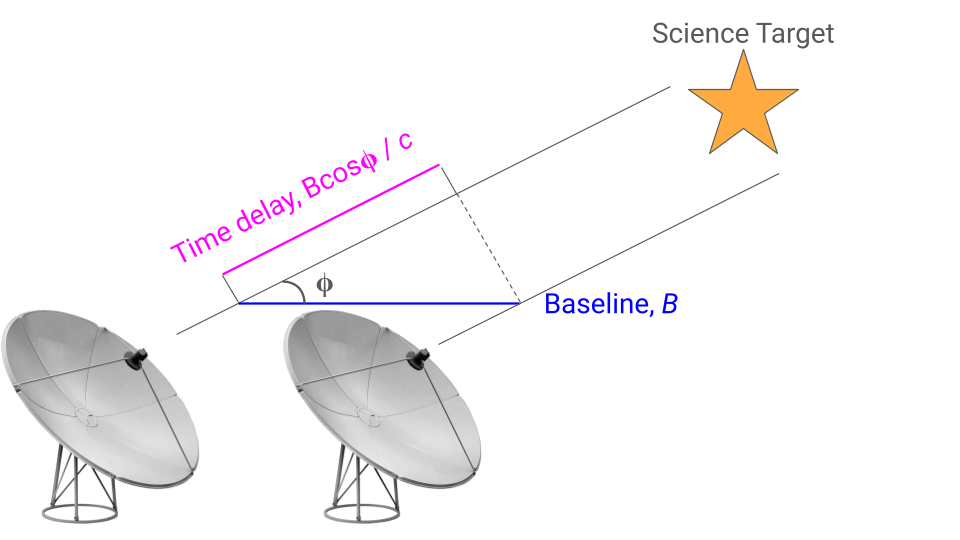
\includegraphics[width=0.7\textwidth]{WRITEUP_AND_IMAGES/IMAGES/WRITEUP/Inter & Data/Schematic_v1.png}
    \caption[Schematic of a two-antenna radio interferometer.]{Schematic of a two-antenna ratio interferometer highlighting the time delay between the signals received at the two antenna.}
    \label{fig: path-delay}
\end{figure}
% ------------------------------------------------



% ------------------------------------------------
\section{UV Plane}
% ------------------------------------------------


The projected baseline between two antennas is decomposed into two coordinates $ (u, v) $ with units of length along the east and north directions, respectively, as projected in the direction of the target. An additional coordinate is $w$, which is the component along the line of sight. Figure \ref{fig: UV-plane} illustrates the geometric relationship between the source direction and projected baseline coordinates. 

For ground-based observing (like ALMA), the object moves across the sky as the Earth rotates, so the $(u, v)$ coverage changes with time. This is beneficial since Earth's rotation increases the $(u,v)$ coverage without requiring additional telescopes \citep{Monnier}. Figure \ref{fig: UV-coverage} shows an example (u,v) coverage for one of the \bfour observations in this study. 



\begin{figure}[htbp]
  \centering
  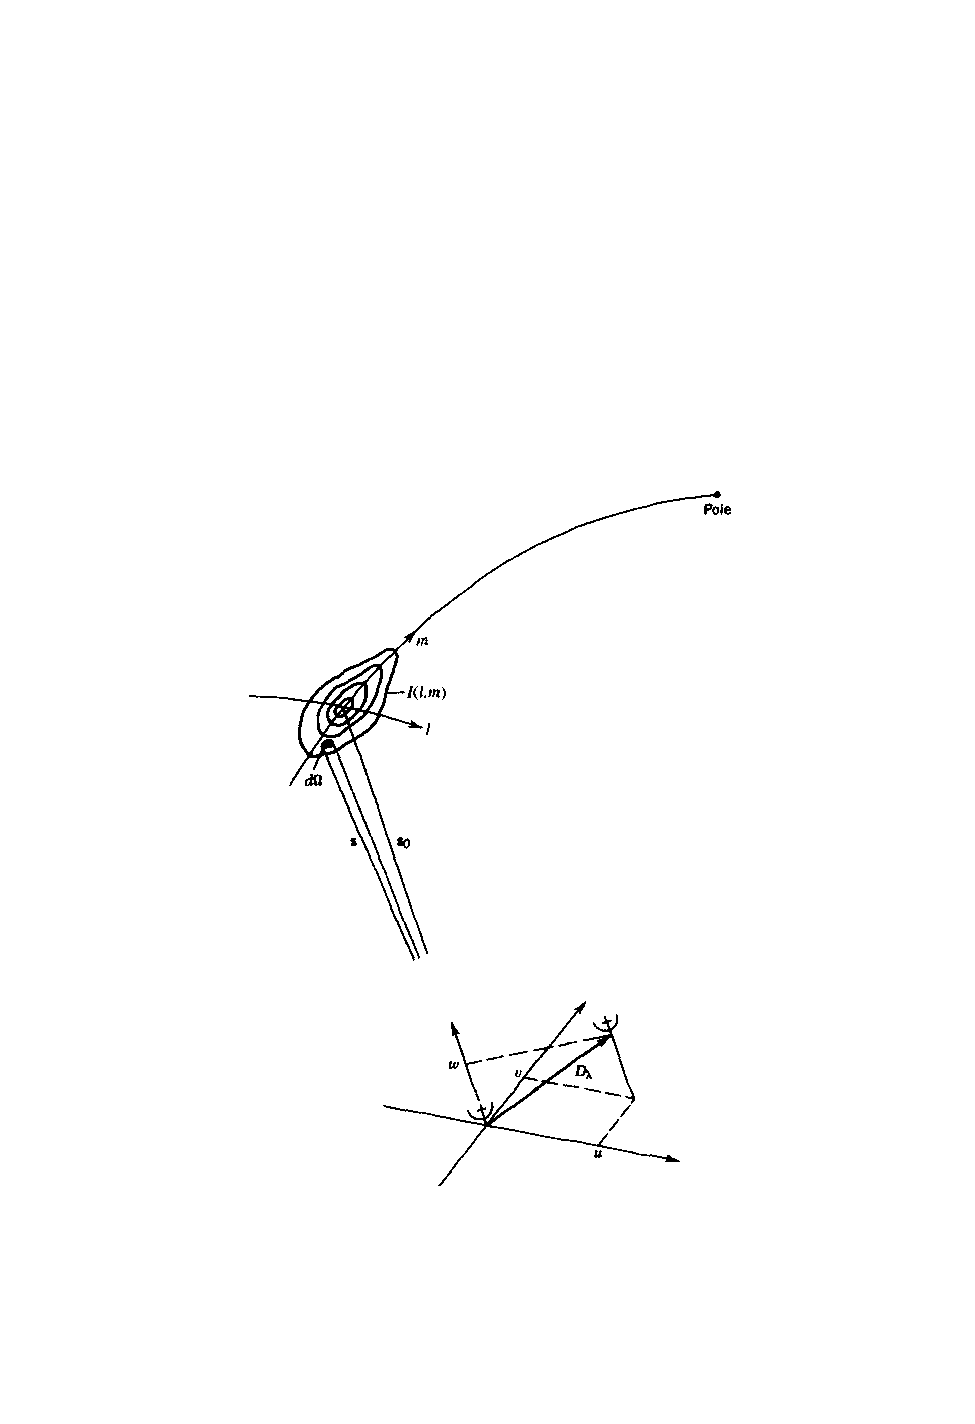
\includegraphics[width=0.75\textwidth]{WRITEUP_AND_IMAGES/IMAGES/WRITEUP/Inter & Data/Thompson.pdf}
  \caption[\note{add short caption after plot is finalized}]{Schematic showing the geometric relationship between a source with sky coordinates $(l, m)$ and the baseline vector of an interferometer, denoted by $D_\lambda$. The baseline is described by its components $(u, v, w)$. Image from \cite{Thompson}, reproduced with permission. \SC{here may be a better image out there.}}
  \label{fig: UV-plane}
\end{figure}



\begin{figure}[htbp]
  \centering
  \includegraphics[width=0.5\textwidth]{WRITEUP_AND_IMAGES/IMAGES/WRITEUP/Inter & Data/UVcoverage_Band4.png}
  \caption[\uv coverage for the \bfour observations.]{Schematic showing the \uv coverage for the \bfour observations. \later{I don't love how this saved, I can add my own axes so its an all white background.}}
  \label{fig: UV-coverage}
\end{figure}



Each antenna pair measures one complex visibility, which describes the amplitude and phase of the interference pattern as a function of time and frequency \citep{Ricci2017}. Each complex visibility samples a single Fourier component of the sky brightness distribution, and the visibilities collectively sample its Fourier transform. The visibility function  $V(u, v) $ is given by:
\begin{equation}
    V(u, v) = \int_{-\infty}^{\infty} I(l, m) e^{-2\pi i(ul + vm)} dl dm
    \label{eq: V(u,v)}
\end{equation}
\noindent where $I(l, m)$ is the intensity function, and $(l, m)$ are the angular sky coordinates  \citep{Marvil2026}. 


% ------------------------------------------------



% ------------------------------------------------
\section{Calibration}
% ------------------------------------------------

Calibration is the process of removing the effects of instrumental and atmospheric factors from visibility data before they are combined into an image. This is achieved by observing a calibration source, an object with well-known properties. Different calibration steps require calibrators with different properties, such as brightness, size, and close proximity to the science target. Before calibration begins, contaminated data from random glitches or other bad data values are flagged and removed to make calibration as effective as possible \citep{Thompson}.



The first step of the calibration process is bandpass calibration, which corrects for frequency-dependent instrumental effects \citep{CASA2012,Ricci2017}. The best calibrator source for this is a very bright quasar with a flat spectrum. The bandpass calibrator does not need to be located near the science target \citep{Bendo2026}.


The next step is flux calibration, which scales the relative amplitudes to the correct flux density scale. A good flux calibrator is a source with a well-known flux density, usually a Solar System object or quasar \citep{Ricci2017}.


The last step is phase and amplitude gain calibration, which corrects time-dependent atmospheric and instrumental variations during the observation. A bright, point-like quasar close to the science target is used as a gain calibrator, as it is observed frequently throughout the observations and needs to capture the atmospheric conditions toward the target \citep{Ricci2017}. 




Since the data presented in this thesis require full polarization, the observations included a polarization calibrator to correct for instrumental polarization or leakage. These objects are typically unpolarized quasars that are observed over several hours at a range of elevations to measure how the instrumental polarization changes with elevation \citep{ALMATechnicalHandbook}.

% ------------------------------------------------



% ------------------------------------------------
\section{Imaging}
% ------------------------------------------------


% ------------------------------------------------
\subsection{Image Reconstruction}
% ------------------------------------------------
To covert the visibilities into an image, we must apply an inverse Fourier transform of the complex visibilities given in Equation \ref{eq: V(u,v)}.  This inverse Fourier transform is \citep{Thompson}:
\begin{equation}
    I(l,m) = \int_{-\infty}^\infty V(u,v) e^{2\pi i(ul+vm)}dudv.
    \label{eq: I(l, m)}
\end{equation}
\noindent Since the \uv coverage is incomplete, applying Equation \ref{eq: I(l, m)} produces a `dirty image', rather than a reconstruction. The dirty image is the true sky brightness distribution convolved with the point spread function of the interferometer, called the `dirty beam' \citep{Marvil2026}.
% ------------------------------------------------



% ------------------------------------------------
\subsection{Deconvolution (\texttt{clean}) and Weighting Schemes}
\label{sec: inter_weighting}
% ------------------------------------------------
Deconvolution is the process of reducing the effects of the dirty beam in the dirty image, typically using the algorithm \clean \citep{Thompson, Marvil2026}. The \clean algorithm iteratively builds a model of the image from delta functions or small Gaussian components. At each iteration, the brightest point of the dirty image is located, a scaled copy of the dirty beam centred on this point is subtracted, and the position and brightness are recorded as \clean components \citep{Monnier}. This process is repeated iteratively until only the residual noise is left. The \clean model is then convolved with the final \clean beam, called the synthesized beam, which is a smooth Gaussian with the same full width at half maximum (FWHM) as the dirty beam. The residual image is added to the restored image, producing the final \clean image \citep{Thompson}. An example of a dirty versus clean image can be seen in Figure \ref{fig: Dirty_vs_clean}. 


\begin{figure}[htbp]
  \centering
  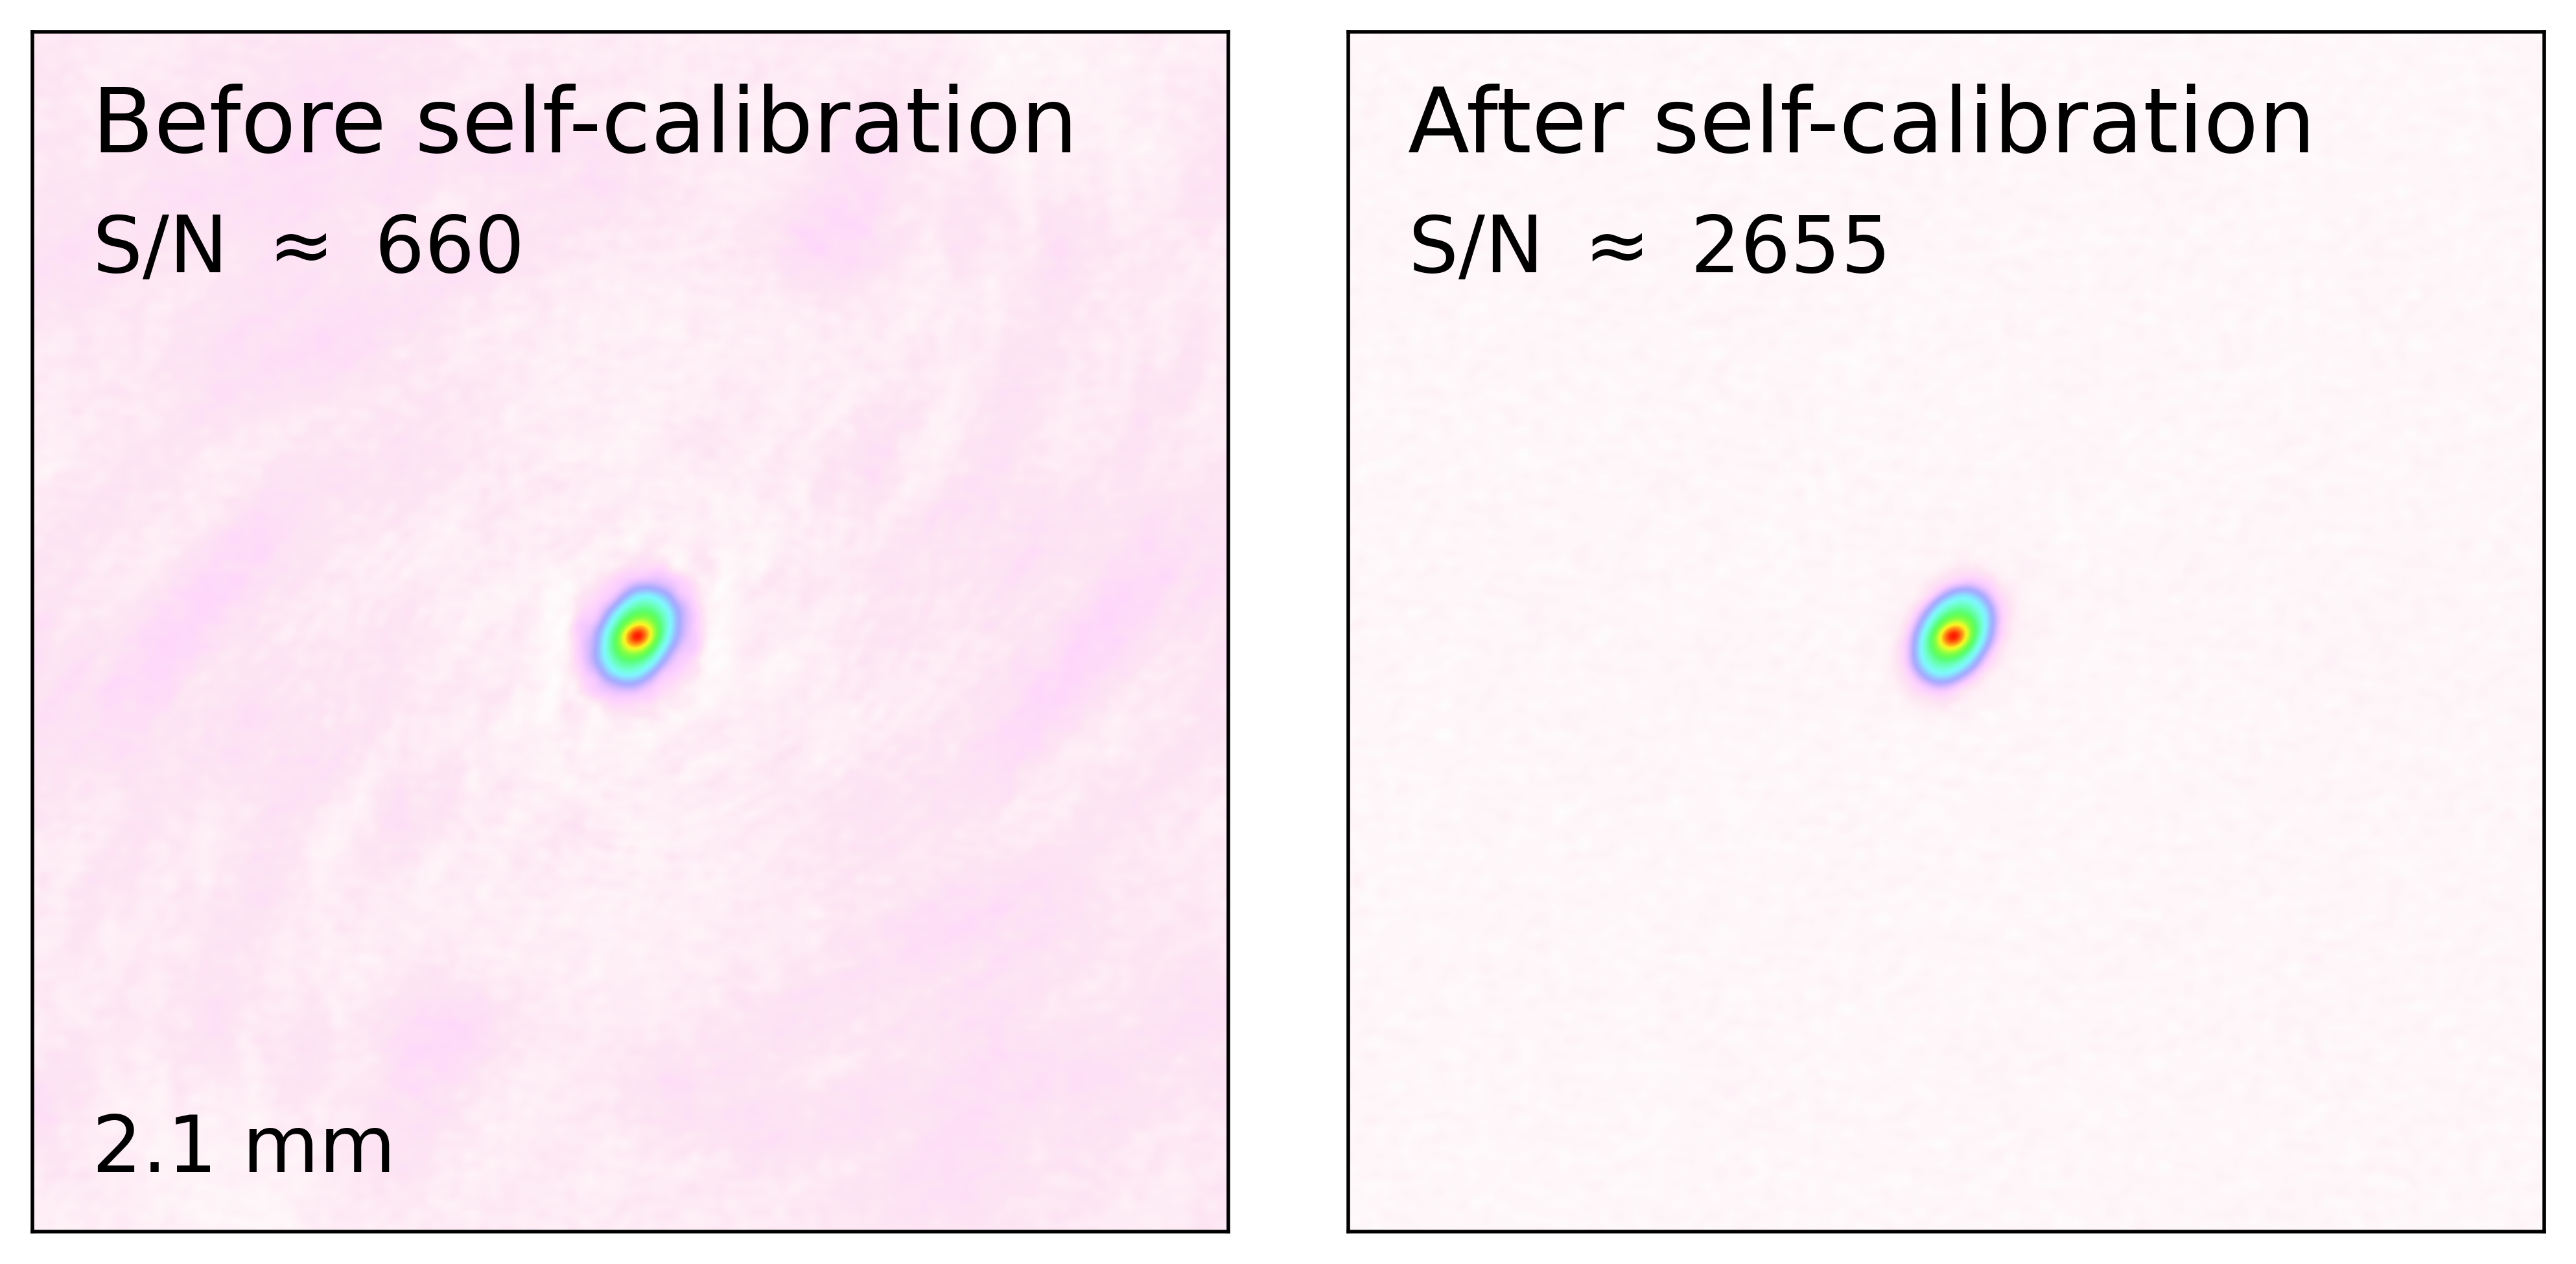
\includegraphics[width=0.99\textwidth]{WRITEUP_AND_IMAGES/IMAGES/WRITEUP/BeforeAndAfterClean.png}
  \caption[\note{add short caption after plot is finalized}]{\note{THIS IS NOT THE REAL IMAGE! Just a placeholder for formatting purposes.}\question{Do I have access to a pre-clean image of IRS 63 or is this something I will need to get from a different source? (I will add a caption too).}}
  \label{fig: Dirty_vs_clean}
\end{figure}




When using the \texttt{clean} algorithm, each visibility in the \uv plane is assigned a weight, which influences the properties of the dirty beam and the resulting image \citep{Marvil2026}. When each visibility is weighted equally, this is called \emph{natural weighting}, which gives the highest sensitivity and therefore best signal-to-noise ratio (\SNRns) for detecting faint objects but with a lower resolution \citep{Monnier, Thompson}. When visibilities are weighted by visibility density in the \uv plane, such that well-sampled regions are given less weight than less-sampled regions, this is called \emph{uniform weighting}. Since the \uv plane is generally more densely sampled at shorter \uv distances, uniform weighting weighs the longer \uv distances higher. This weighting produces a smaller synthesized beam and therefore higher angular resolution, but with lower sensitivity as a trade-off \citep{Monnier}.


A `robust' parameter was introduced in \cite{briggs} for a weighting scheme called Briggs weighting. The robust parameter controls a balance between natural and uniform weighting to find an ideal trade-off between sensitivity and angular resolution \citep{Monnier, Marvil2026}. The robust parameter ranges from -2 to 2, where more negative values have weighting closer to uniform weighting, and more positive values produce weighting closer to natural weighting \citep{Thompson}.
% ------------------------------------------------





% ------------------------------------------------
\subsection{Self-Calibration}
% ------------------------------------------------
Self-calibration is an additional calibration step that can be performed after standard calibration. In standard calibration, calibration sources such as quasars are used to determine instrumental and atmospheric effects. In self-calibration, the science target itself is used as the calibrator to further correct both the phase and amplitude of the data. Because of this, the target needs to be bright, with a \SNR $\gtrsim$ 100. 


The signal received by each antenna can be affected by time-dependent atmospheric variations, which can introduce additional calibration errors. Self-calibration is useful for reducing artifacts caused by these errors, as well as artifacts from a background source due to direction-independent calibration errors \citep{Marvil2}. The specific details on the self-calibration process used in this project are described in Chapter \ref{ch_data}. 
% ------------------------------------------------
